\documentclass[twoside]{book}

% Packages required by doxygen
\usepackage{fixltx2e}
\usepackage{calc}
\usepackage{doxygen}
\usepackage[export]{adjustbox} % also loads graphicx
\usepackage{graphicx}
\usepackage[utf8]{inputenc}
\usepackage{makeidx}
\usepackage{multicol}
\usepackage{multirow}
\PassOptionsToPackage{warn}{textcomp}
\usepackage{textcomp}
\usepackage[nointegrals]{wasysym}
\usepackage[table]{xcolor}

% Font selection
\usepackage[T1]{fontenc}
\usepackage[scaled=.90]{helvet}
\usepackage{courier}
\usepackage{amssymb}
\usepackage{sectsty}
\renewcommand{\familydefault}{\sfdefault}
\allsectionsfont{%
  \fontseries{bc}\selectfont%
  \color{darkgray}%
}
\renewcommand{\DoxyLabelFont}{%
  \fontseries{bc}\selectfont%
  \color{darkgray}%
}
\newcommand{\+}{\discretionary{\mbox{\scriptsize$\hookleftarrow$}}{}{}}

% Page & text layout
\usepackage{geometry}
\geometry{%
  a4paper,%
  top=2.5cm,%
  bottom=2.5cm,%
  left=2.5cm,%
  right=2.5cm%
}
\tolerance=750
\hfuzz=15pt
\hbadness=750
\setlength{\emergencystretch}{15pt}
\setlength{\parindent}{0cm}
\setlength{\parskip}{3ex plus 2ex minus 2ex}
\makeatletter
\renewcommand{\paragraph}{%
  \@startsection{paragraph}{4}{0ex}{-1.0ex}{1.0ex}{%
    \normalfont\normalsize\bfseries\SS@parafont%
  }%
}
\renewcommand{\subparagraph}{%
  \@startsection{subparagraph}{5}{0ex}{-1.0ex}{1.0ex}{%
    \normalfont\normalsize\bfseries\SS@subparafont%
  }%
}
\makeatother

% Headers & footers
\usepackage{fancyhdr}
\pagestyle{fancyplain}
\fancyhead[LE]{\fancyplain{}{\bfseries\thepage}}
\fancyhead[CE]{\fancyplain{}{}}
\fancyhead[RE]{\fancyplain{}{\bfseries\leftmark}}
\fancyhead[LO]{\fancyplain{}{\bfseries\rightmark}}
\fancyhead[CO]{\fancyplain{}{}}
\fancyhead[RO]{\fancyplain{}{\bfseries\thepage}}
\fancyfoot[LE]{\fancyplain{}{}}
\fancyfoot[CE]{\fancyplain{}{}}
\fancyfoot[RE]{\fancyplain{}{\bfseries\scriptsize Generated by Doxygen }}
\fancyfoot[LO]{\fancyplain{}{\bfseries\scriptsize Generated by Doxygen }}
\fancyfoot[CO]{\fancyplain{}{}}
\fancyfoot[RO]{\fancyplain{}{}}
\renewcommand{\footrulewidth}{0.4pt}
\renewcommand{\chaptermark}[1]{%
  \markboth{#1}{}%
}
\renewcommand{\sectionmark}[1]{%
  \markright{\thesection\ #1}%
}

% Indices & bibliography
\usepackage{natbib}
\usepackage[titles]{tocloft}
\setcounter{tocdepth}{3}
\setcounter{secnumdepth}{5}
\makeindex

% Hyperlinks (required, but should be loaded last)
\usepackage{ifpdf}
\ifpdf
  \usepackage[pdftex,pagebackref=true]{hyperref}
\else
  \usepackage[ps2pdf,pagebackref=true]{hyperref}
\fi
\hypersetup{%
  colorlinks=true,%
  linkcolor=blue,%
  citecolor=blue,%
  unicode%
}

% Custom commands
\newcommand{\clearemptydoublepage}{%
  \newpage{\pagestyle{empty}\cleardoublepage}%
}

\usepackage{caption}
\captionsetup{labelsep=space,justification=centering,font={bf},singlelinecheck=off,skip=4pt,position=top}

%===== C O N T E N T S =====

\begin{document}

% Titlepage & ToC
\hypersetup{pageanchor=false,
             bookmarksnumbered=true,
             pdfencoding=unicode
            }
\pagenumbering{alph}
\begin{titlepage}
\vspace*{7cm}
\begin{center}%
{\Large N\+TP Library \\[1ex]\large 1 }\\
\vspace*{1cm}
{\large Generated by Doxygen 1.8.13}\\
\end{center}
\end{titlepage}
\clearemptydoublepage
\pagenumbering{roman}
\tableofcontents
\clearemptydoublepage
\pagenumbering{arabic}
\hypersetup{pageanchor=true}

%--- Begin generated contents ---
\chapter{Class Index}
\section{Class List}
Here are the classes, structs, unions and interfaces with brief descriptions\+:\begin{DoxyCompactList}
\item\contentsline{section}{\hyperlink{structconfiguration__t}{configuration\+\_\+t} \\*E\+E\+P\+R\+OM saved configuration }{\pageref{structconfiguration__t}}{}
\end{DoxyCompactList}

\chapter{File Index}
\section{File List}
Here is a list of all documented files with brief descriptions\+:\begin{DoxyCompactList}
\item\contentsline{section}{sketchbook/libraries/\+Digiteco\+Power/\hyperlink{digiteco__power_8cpp}{digiteco\+\_\+power.\+cpp} }{\pageref{digiteco__power_8cpp}}{}
\item\contentsline{section}{sketchbook/libraries/\+Digiteco\+Power/\hyperlink{digiteco__power_8h}{digiteco\+\_\+power.\+h} }{\pageref{digiteco__power_8h}}{}
\item\contentsline{section}{sketchbook/libraries/\+H\+Y\+T2\+X1/\hyperlink{hyt2x1_8cpp}{hyt2x1.\+cpp} }{\pageref{hyt2x1_8cpp}}{}
\item\contentsline{section}{sketchbook/libraries/\+H\+Y\+T2\+X1/\hyperlink{hyt2x1_8h}{hyt2x1.\+h} }{\pageref{hyt2x1_8h}}{}
\item\contentsline{section}{sketchbook/libraries/\+N\+T\+P/\hyperlink{ntp_8cpp}{ntp.\+cpp} }{\pageref{ntp_8cpp}}{}
\item\contentsline{section}{sketchbook/libraries/\+N\+T\+P/\hyperlink{ntp_8h}{ntp.\+h} }{\pageref{ntp_8h}}{}
\item\contentsline{section}{sketchbook/libraries/\+P\+C\+F8563/\hyperlink{pcf8563_8cpp}{pcf8563.\+cpp} }{\pageref{pcf8563_8cpp}}{}
\item\contentsline{section}{sketchbook/libraries/\+P\+C\+F8563/\hyperlink{pcf8563_8h}{pcf8563.\+h} }{\pageref{pcf8563_8h}}{}
\item\contentsline{section}{sketchbook/libraries/\+Rmap/\hyperlink{debug_8cpp}{debug.\+cpp} }{\pageref{debug_8cpp}}{}
\item\contentsline{section}{sketchbook/libraries/\+Rmap/\hyperlink{debug_8h}{debug.\+h} }{\pageref{debug_8h}}{}
\item\contentsline{section}{sketchbook/libraries/\+Rmap/\hyperlink{eeprom__utility_8h}{eeprom\+\_\+utility.\+h} }{\pageref{eeprom__utility_8h}}{}
\item\contentsline{section}{sketchbook/libraries/\+Rmap/\hyperlink{i2c__utility_8cpp}{i2c\+\_\+utility.\+cpp} }{\pageref{i2c__utility_8cpp}}{}
\item\contentsline{section}{sketchbook/libraries/\+Rmap/\hyperlink{i2c__utility_8h}{i2c\+\_\+utility.\+h} }{\pageref{i2c__utility_8h}}{}
\item\contentsline{section}{sketchbook/libraries/\+Rmap/\hyperlink{registers-rain_8h}{registers-\/rain.\+h} }{\pageref{registers-rain_8h}}{}
\item\contentsline{section}{sketchbook/libraries/\+Rmap/\hyperlink{registers-th_8h}{registers-\/th.\+h} }{\pageref{registers-th_8h}}{}
\item\contentsline{section}{sketchbook/libraries/\+Rmap/\hyperlink{registers_8h}{registers.\+h} }{\pageref{registers_8h}}{}
\item\contentsline{section}{sketchbook/libraries/\+Rmap/\hyperlink{rmap__utility_8cpp}{rmap\+\_\+utility.\+cpp} }{\pageref{rmap__utility_8cpp}}{}
\item\contentsline{section}{sketchbook/libraries/\+Rmap/\hyperlink{rmap__utility_8h}{rmap\+\_\+utility.\+h} }{\pageref{rmap__utility_8h}}{}
\item\contentsline{section}{sketchbook/libraries/\+Rmap/\hyperlink{sdcard__utility_8cpp}{sdcard\+\_\+utility.\+cpp} }{\pageref{sdcard__utility_8cpp}}{}
\item\contentsline{section}{sketchbook/libraries/\+Rmap/\hyperlink{sdcard__utility_8h}{sdcard\+\_\+utility.\+h} }{\pageref{sdcard__utility_8h}}{}
\item\contentsline{section}{sketchbook/libraries/\+Rmap/\hyperlink{stima__module_8h}{stima\+\_\+module.\+h} }{\pageref{stima__module_8h}}{}
\item\contentsline{section}{sketchbook/libraries/\+Rmap/\hyperlink{typedef_8h}{typedef.\+h} }{\pageref{typedef_8h}}{}
\item\contentsline{section}{sketchbook/libraries/\+Rmap\+Config/\hyperlink{debug__config_8h}{debug\+\_\+config.\+h} }{\pageref{debug__config_8h}}{}
\item\contentsline{section}{sketchbook/libraries/\+Rmap\+Config/\hyperlink{ethernet__config_8h}{ethernet\+\_\+config.\+h} }{\pageref{ethernet__config_8h}}{}
\item\contentsline{section}{sketchbook/libraries/\+Rmap\+Config/\hyperlink{gsm__config_8h}{gsm\+\_\+config.\+h} }{\pageref{gsm__config_8h}}{}
\item\contentsline{section}{sketchbook/libraries/\+Rmap\+Config/\hyperlink{hardware__config_8h}{hardware\+\_\+config.\+h} }{\pageref{hardware__config_8h}}{}
\item\contentsline{section}{sketchbook/libraries/\+Rmap\+Config/\hyperlink{json__config_8h}{json\+\_\+config.\+h} }{\pageref{json__config_8h}}{}
\item\contentsline{section}{sketchbook/libraries/\+Rmap\+Config/\hyperlink{lcd__config_8h}{lcd\+\_\+config.\+h} }{\pageref{lcd__config_8h}}{}
\item\contentsline{section}{sketchbook/libraries/\+Rmap\+Config/\hyperlink{mqtt__config_8h}{mqtt\+\_\+config.\+h} }{\pageref{mqtt__config_8h}}{}
\item\contentsline{section}{sketchbook/libraries/\+Rmap\+Config/\hyperlink{ntp__config_8h}{ntp\+\_\+config.\+h} }{\pageref{ntp__config_8h}}{}
\item\contentsline{section}{sketchbook/libraries/\+Rmap\+Config/\hyperlink{sdcard__config_8h}{sdcard\+\_\+config.\+h} }{\pageref{sdcard__config_8h}}{}
\item\contentsline{section}{sketchbook/libraries/\+Rmap\+Config/\hyperlink{sensors__config_8h}{sensors\+\_\+config.\+h} }{\pageref{sensors__config_8h}}{}
\item\contentsline{section}{sketchbook/libraries/\+Sensor\+Driver/\hyperlink{SensorDriver_8cpp}{Sensor\+Driver.\+cpp} }{\pageref{SensorDriver_8cpp}}{}
\item\contentsline{section}{sketchbook/libraries/\+Sensor\+Driver/\hyperlink{SensorDriver_8h}{Sensor\+Driver.\+h} }{\pageref{SensorDriver_8h}}{}
\item\contentsline{section}{sketchbook/libraries/\+Sensor\+Driver/\hyperlink{SensorDriverSensors_8h}{Sensor\+Driver\+Sensors.\+h} }{\pageref{SensorDriverSensors_8h}}{}
\item\contentsline{section}{sketchbook/libraries/sim800/\hyperlink{sim800_8cpp}{sim800.\+cpp} }{\pageref{sim800_8cpp}}{}
\item\contentsline{section}{sketchbook/libraries/sim800/\hyperlink{sim800_8h}{sim800.\+h} }{\pageref{sim800_8h}}{}
\item\contentsline{section}{sketchbook/libraries/sim800/\hyperlink{sim800Client_8h}{sim800\+Client.\+h} }{\pageref{sim800Client_8h}}{}
\item\contentsline{section}{sketchbook/rmap/{\bfseries version.\+h} }{\pageref{version_8h}}{}
\item\contentsline{section}{sketchbook/rmap/i2c-\/rain/\hyperlink{i2c-rain-config_8h}{i2c-\/rain-\/config.\+h} }{\pageref{i2c-rain-config_8h}}{}
\item\contentsline{section}{sketchbook/rmap/i2c-\/rain/\hyperlink{i2c-rain_8h}{i2c-\/rain.\+h} }{\pageref{i2c-rain_8h}}{}
\item\contentsline{section}{sketchbook/rmap/i2c-\/rain/\hyperlink{i2c-rain_8ino}{i2c-\/rain.\+ino} }{\pageref{i2c-rain_8ino}}{}
\item\contentsline{section}{sketchbook/rmap/i2c-\/th/\hyperlink{i2c-th-config_8h}{i2c-\/th-\/config.\+h} }{\pageref{i2c-th-config_8h}}{}
\item\contentsline{section}{sketchbook/rmap/i2c-\/th/\hyperlink{i2c-th_8h}{i2c-\/th.\+h} }{\pageref{i2c-th_8h}}{}
\item\contentsline{section}{sketchbook/rmap/i2c-\/th/\hyperlink{i2c-th_8ino}{i2c-\/th.\+ino} }{\pageref{i2c-th_8ino}}{}
\item\contentsline{section}{sketchbook/rmap/rmap/\hyperlink{rmap-config_8h}{rmap-\/config.\+h} }{\pageref{rmap-config_8h}}{}
\item\contentsline{section}{sketchbook/rmap/rmap/\hyperlink{rmap_8h}{rmap.\+h} }{\pageref{rmap_8h}}{}
\item\contentsline{section}{sketchbook/rmap/rmap/\hyperlink{rmap_8ino}{rmap.\+ino} }{\pageref{rmap_8ino}}{}
\end{DoxyCompactList}

\chapter{Class Documentation}
\hypertarget{classNtp}{}\section{Ntp Class Reference}
\label{classNtp}\index{Ntp@{Ntp}}


\hyperlink{classNtp}{Ntp} class.  




{\ttfamily \#include $<$ntp.\+h$>$}

\subsection*{Static Public Member Functions}
\begin{DoxyCompactItemize}
\item 
static bool \hyperlink{classNtp_a439e0498ea9209f74d91d7cf4d8805b0}{send\+Request} (Ethernet\+U\+DP $\ast$client, const char $\ast$server)
\begin{DoxyCompactList}\small\item\em Send ntp request over ethernet client. \end{DoxyCompactList}\item 
static uint32\+\_\+t \hyperlink{classNtp_a6df9e799d7fb829ff163ea14a70f6999}{get\+Response} (Ethernet\+U\+DP $\ast$client)
\begin{DoxyCompactList}\small\item\em Get ntp response. \end{DoxyCompactList}\item 
static bool \hyperlink{classNtp_a98c5dfc44e09069f5ec607adba8177b2}{send\+Request} (\hyperlink{classsim800Client}{sim800\+Client} $\ast$client)
\begin{DoxyCompactList}\small\item\em Send ntp request over sim800 client. \end{DoxyCompactList}\item 
static uint32\+\_\+t \hyperlink{classNtp_a6456f082f6b3012f72c5064e45791ddd}{get\+Response} (\hyperlink{classsim800Client}{sim800\+Client} $\ast$client)
\begin{DoxyCompactList}\small\item\em Get ntp response. \end{DoxyCompactList}\end{DoxyCompactItemize}


\subsection{Detailed Description}
\hyperlink{classNtp}{Ntp} class. 

\subsection{Member Function Documentation}
\mbox{\Hypertarget{classNtp_a6df9e799d7fb829ff163ea14a70f6999}\label{classNtp_a6df9e799d7fb829ff163ea14a70f6999}} 
\index{Ntp@{Ntp}!get\+Response@{get\+Response}}
\index{get\+Response@{get\+Response}!Ntp@{Ntp}}
\subsubsection{\texorpdfstring{get\+Response()}{getResponse()}\hspace{0.1cm}{\footnotesize\ttfamily [1/2]}}
{\footnotesize\ttfamily uint32\+\_\+t Ntp\+::get\+Response (\begin{DoxyParamCaption}\item[{Ethernet\+U\+DP $\ast$}]{client }\end{DoxyParamCaption})\hspace{0.3cm}{\ttfamily [static]}}



Get ntp response. 


\begin{DoxyParams}[1]{Parameters}
\mbox{\tt in}  & {\em $\ast$client} & ethernet client pointer. \\
\hline
\end{DoxyParams}
\begin{DoxyReturn}{Returns}
ntp time in seconds since 01/01/1970 00\+:0\+:00. 
\end{DoxyReturn}
\mbox{\Hypertarget{classNtp_a6456f082f6b3012f72c5064e45791ddd}\label{classNtp_a6456f082f6b3012f72c5064e45791ddd}} 
\index{Ntp@{Ntp}!get\+Response@{get\+Response}}
\index{get\+Response@{get\+Response}!Ntp@{Ntp}}
\subsubsection{\texorpdfstring{get\+Response()}{getResponse()}\hspace{0.1cm}{\footnotesize\ttfamily [2/2]}}
{\footnotesize\ttfamily uint32\+\_\+t Ntp\+::get\+Response (\begin{DoxyParamCaption}\item[{\hyperlink{classsim800Client}{sim800\+Client} $\ast$}]{client }\end{DoxyParamCaption})\hspace{0.3cm}{\ttfamily [static]}}



Get ntp response. 


\begin{DoxyParams}[1]{Parameters}
\mbox{\tt in}  & {\em $\ast$client} & sim800 client pointer. \\
\hline
\end{DoxyParams}
\begin{DoxyReturn}{Returns}
ntp time in seconds since 01/01/1970 00\+:0\+:00. 
\end{DoxyReturn}
\mbox{\Hypertarget{classNtp_a439e0498ea9209f74d91d7cf4d8805b0}\label{classNtp_a439e0498ea9209f74d91d7cf4d8805b0}} 
\index{Ntp@{Ntp}!send\+Request@{send\+Request}}
\index{send\+Request@{send\+Request}!Ntp@{Ntp}}
\subsubsection{\texorpdfstring{send\+Request()}{sendRequest()}\hspace{0.1cm}{\footnotesize\ttfamily [1/2]}}
{\footnotesize\ttfamily bool Ntp\+::send\+Request (\begin{DoxyParamCaption}\item[{Ethernet\+U\+DP $\ast$}]{client,  }\item[{const char $\ast$}]{server }\end{DoxyParamCaption})\hspace{0.3cm}{\ttfamily [static]}}



Send ntp request over ethernet client. 


\begin{DoxyParams}[1]{Parameters}
\mbox{\tt in}  & {\em $\ast$client} & ethernet client pointer. \\
\hline
\mbox{\tt in}  & {\em $\ast$server} & ntp server. \\
\hline
\end{DoxyParams}
\begin{DoxyReturn}{Returns}
true if request was sent. 
\end{DoxyReturn}
\mbox{\Hypertarget{classNtp_a98c5dfc44e09069f5ec607adba8177b2}\label{classNtp_a98c5dfc44e09069f5ec607adba8177b2}} 
\index{Ntp@{Ntp}!send\+Request@{send\+Request}}
\index{send\+Request@{send\+Request}!Ntp@{Ntp}}
\subsubsection{\texorpdfstring{send\+Request()}{sendRequest()}\hspace{0.1cm}{\footnotesize\ttfamily [2/2]}}
{\footnotesize\ttfamily bool Ntp\+::send\+Request (\begin{DoxyParamCaption}\item[{\hyperlink{classsim800Client}{sim800\+Client} $\ast$}]{client }\end{DoxyParamCaption})\hspace{0.3cm}{\ttfamily [static]}}



Send ntp request over sim800 client. 


\begin{DoxyParams}[1]{Parameters}
\mbox{\tt in}  & {\em $\ast$client} & sim800 client pointer. \\
\hline
\end{DoxyParams}
\begin{DoxyReturn}{Returns}
true if request was sent. 
\end{DoxyReturn}


The documentation for this class was generated from the following files\+:\begin{DoxyCompactItemize}
\item 
sketchbook/libraries/\+N\+T\+P/\hyperlink{ntp_8h}{ntp.\+h}\item 
sketchbook/libraries/\+N\+T\+P/\hyperlink{ntp_8cpp}{ntp.\+cpp}\end{DoxyCompactItemize}

\chapter{File Documentation}
\hypertarget{ntp_8cpp}{}\section{sketchbook/libraries/\+N\+T\+P/ntp.cpp File Reference}
\label{ntp_8cpp}\index{sketchbook/libraries/\+N\+T\+P/ntp.\+cpp@{sketchbook/libraries/\+N\+T\+P/ntp.\+cpp}}
{\ttfamily \#include \char`\"{}ntp.\+h\char`\"{}}\newline
Include dependency graph for ntp.\+cpp\+:
\nopagebreak
\begin{figure}[H]
\begin{center}
\leavevmode
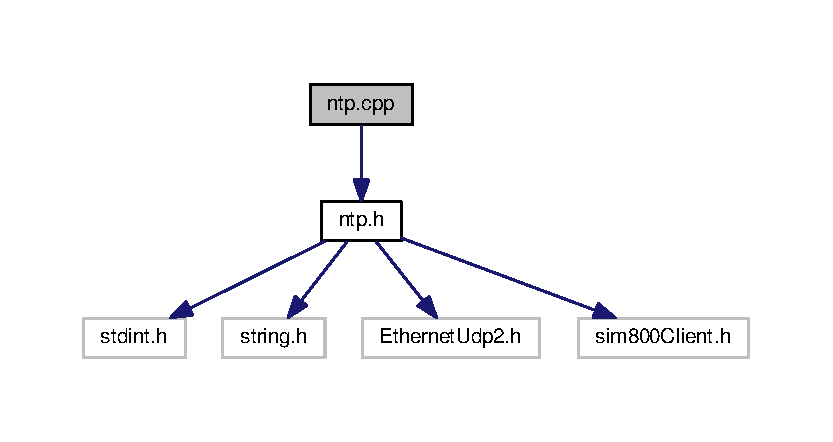
\includegraphics[width=350pt]{ntp_8cpp__incl}
\end{center}
\end{figure}

\hypertarget{ntp_8h}{}\section{sketchbook/libraries/\+N\+T\+P/ntp.h File Reference}
\label{ntp_8h}\index{sketchbook/libraries/\+N\+T\+P/ntp.\+h@{sketchbook/libraries/\+N\+T\+P/ntp.\+h}}
{\ttfamily \#include $<$stdint.\+h$>$}\newline
{\ttfamily \#include $<$string.\+h$>$}\newline
{\ttfamily \#include $<$Ethernet\+Udp2.\+h$>$}\newline
{\ttfamily \#include $<$sim800\+Client.\+h$>$}\newline
Include dependency graph for ntp.\+h\+:
\nopagebreak
\begin{figure}[H]
\begin{center}
\leavevmode
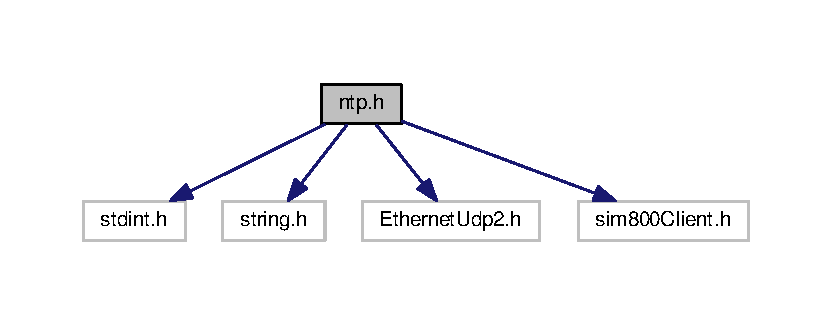
\includegraphics[width=350pt]{ntp_8h__incl}
\end{center}
\end{figure}
This graph shows which files directly or indirectly include this file\+:
\nopagebreak
\begin{figure}[H]
\begin{center}
\leavevmode
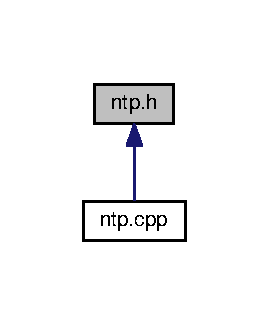
\includegraphics[width=318pt]{ntp_8h__dep__incl}
\end{center}
\end{figure}
\subsection*{Classes}
\begin{DoxyCompactItemize}
\item 
class \hyperlink{classNtp}{Ntp}
\begin{DoxyCompactList}\small\item\em \hyperlink{classNtp}{Ntp} class. \end{DoxyCompactList}\end{DoxyCompactItemize}
\subsection*{Macros}
\begin{DoxyCompactItemize}
\item 
\mbox{\Hypertarget{ntp_8h_a57df452a6d54697643631ce3039623d4}\label{ntp_8h_a57df452a6d54697643631ce3039623d4}} 
\#define \hyperlink{ntp_8h_a57df452a6d54697643631ce3039623d4}{N\+T\+P\+\_\+\+S\+E\+R\+V\+E\+R\+\_\+\+P\+O\+RT}~(123)
\begin{DoxyCompactList}\small\item\em N\+TP server port. \end{DoxyCompactList}\item 
\mbox{\Hypertarget{ntp_8h_aa1c0658c928d132f60e25b16771be754}\label{ntp_8h_aa1c0658c928d132f60e25b16771be754}} 
\#define \hyperlink{ntp_8h_aa1c0658c928d132f60e25b16771be754}{N\+T\+P\+\_\+\+P\+A\+C\+K\+E\+T\+\_\+\+L\+E\+N\+G\+TH}~(48)
\begin{DoxyCompactList}\small\item\em N\+TP packet length. \end{DoxyCompactList}\item 
\mbox{\Hypertarget{ntp_8h_ace39986119607151c9b16cecf698abe1}\label{ntp_8h_ace39986119607151c9b16cecf698abe1}} 
\#define \hyperlink{ntp_8h_ace39986119607151c9b16cecf698abe1}{N\+T\+P\+\_\+\+R\+E\+C\+E\+I\+V\+E\+\_\+\+T\+I\+M\+E\+S\+T\+A\+M\+P\+\_\+\+O\+F\+F\+S\+ET}~(40)
\begin{DoxyCompactList}\small\item\em N\+TP received timestamp offset. \end{DoxyCompactList}\item 
\mbox{\Hypertarget{ntp_8h_a7c6347c9dc2a84fc9f90d6eaca9df2ca}\label{ntp_8h_a7c6347c9dc2a84fc9f90d6eaca9df2ca}} 
\#define \hyperlink{ntp_8h_a7c6347c9dc2a84fc9f90d6eaca9df2ca}{N\+T\+P\+\_\+1\+\_\+\+H\+O\+U\+R\+\_\+\+S\+E\+C\+O\+N\+DS}~(3600\+U\+L)
\begin{DoxyCompactList}\small\item\em seconds in one hour. \end{DoxyCompactList}\item 
\mbox{\Hypertarget{ntp_8h_a2805f547f7dc24f8477827a4120d7385}\label{ntp_8h_a2805f547f7dc24f8477827a4120d7385}} 
\#define \hyperlink{ntp_8h_a2805f547f7dc24f8477827a4120d7385}{N\+T\+P\+\_\+70\+\_\+\+Y\+E\+A\+R\+S\+\_\+\+S\+E\+C\+O\+N\+DS}~(2208988800\+U\+L)
\begin{DoxyCompactList}\small\item\em seconds in 70 years. \end{DoxyCompactList}\item 
\mbox{\Hypertarget{ntp_8h_a004ce391c29e30cea2c3f958adfd009e}\label{ntp_8h_a004ce391c29e30cea2c3f958adfd009e}} 
\#define \hyperlink{ntp_8h_a004ce391c29e30cea2c3f958adfd009e}{N\+T\+P\+\_\+\+V\+A\+L\+I\+D\+\_\+\+S\+T\+A\+R\+T\+\_\+\+T\+I\+M\+E\+\_\+S}~(1483228800\+U\+L)
\begin{DoxyCompactList}\small\item\em seconds for 00\+:00\+:00 01/01/2017 since 00\+:00\+:00 01/01/1970. \end{DoxyCompactList}\item 
\mbox{\Hypertarget{ntp_8h_a812dbabea90c19f0a440aeeb8d20fce3}\label{ntp_8h_a812dbabea90c19f0a440aeeb8d20fce3}} 
\#define \hyperlink{ntp_8h_a812dbabea90c19f0a440aeeb8d20fce3}{N\+T\+P\+\_\+\+T\+I\+M\+E\+Z\+O\+NE}~(1)
\begin{DoxyCompactList}\small\item\em N\+TP timezone. \end{DoxyCompactList}\end{DoxyCompactItemize}

%--- End generated contents ---

% Index
\backmatter
\newpage
\phantomsection
\clearemptydoublepage
\addcontentsline{toc}{chapter}{Index}
\printindex

\end{document}
